
分子生物学的核心是中心法则(\autoref{fig:genetic_central_dogma})。除此之外,朊病毒通过催化其他正常蛋白质发生构象变化来实现“复制”,和传统意义的复制不太一样。

对于分子生物学的知识,原核生物重点记忆,真核生物关注和原核生物的不同点,古菌了解即可。

\begin{figure}[htbp]
	\centering
	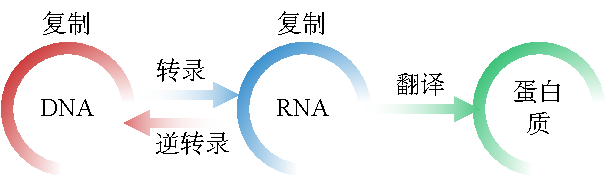
\includegraphics{中心法则.pdf}
	\caption{中心法则}
	\label{fig:genetic_central_dogma}
\end{figure}


\section{DNA复制}

\subsection{DNA复制的一般特征}

DNA复制的一般特征包括:

\begin{description}
	\item[需要模板、dNTPs、\ce{Mg^{2+}}] 其中\ce{Mg^{2+}}的作用是屏蔽磷酸基团的负电荷。有时少量的dUTP会掺入DNA。
	\item[模板DNA需要解链] 暴露出在双螺旋内部的碱基。
	\item[半保留复制] Meselson和Stahl的实验证明了这一点,注意使用的是\ce{CsCl}平衡密度梯度离心。(\autoref{fig:Meselson和Stahl的证明DNA半保留复制的实验流程})
	\item[通常需引物] 由DNA聚合酶的所致。引物多为RNA,少数为蛋白质,PCR的引物为DNA。一种噬菌体的DNA复制不需要引物。
	\item[复制方向永远是5$\prime$$\longrightarrow$3$\prime$] 可以向复制体系中加入ddNTP来验证。若为5$\prime$$\longrightarrow$3$\prime$,则会掺入ddNTP,进而导致末端终止;若为3$\prime$$\longrightarrow$5$\prime$,则ddNTP根本没机会掺入,复制不终止。
	\item[起点固定] DNA复制的起点即复制起始区。详后。
	\item[多双向,少单向] 从复制子开始向两侧复制,是为双向复制。
	\item[半不连续性] 因dNTP只能5$\prime$$\longrightarrow$3$\prime$加入(\autoref{fig:证明DNA复制方向的实验}),故有前导链、后随链之分。后随链产生冈崎片段。
	\item[高度忠实性] 在进行DNA复制时,细胞内依赖一系列校对与纠错机制来保证DNA复制具有远高于其他核酸合成反应的忠实性。
	\item[高度进行性] 进行性指DNA聚合酶从与模板结合到解离这段时间内,催化DNA分子延长的核苷酸数。参与DNA复制的,一定是细胞内进行性高的DNA聚合酶。
\end{description}

\begin{figure}[htbp]
	\centering
	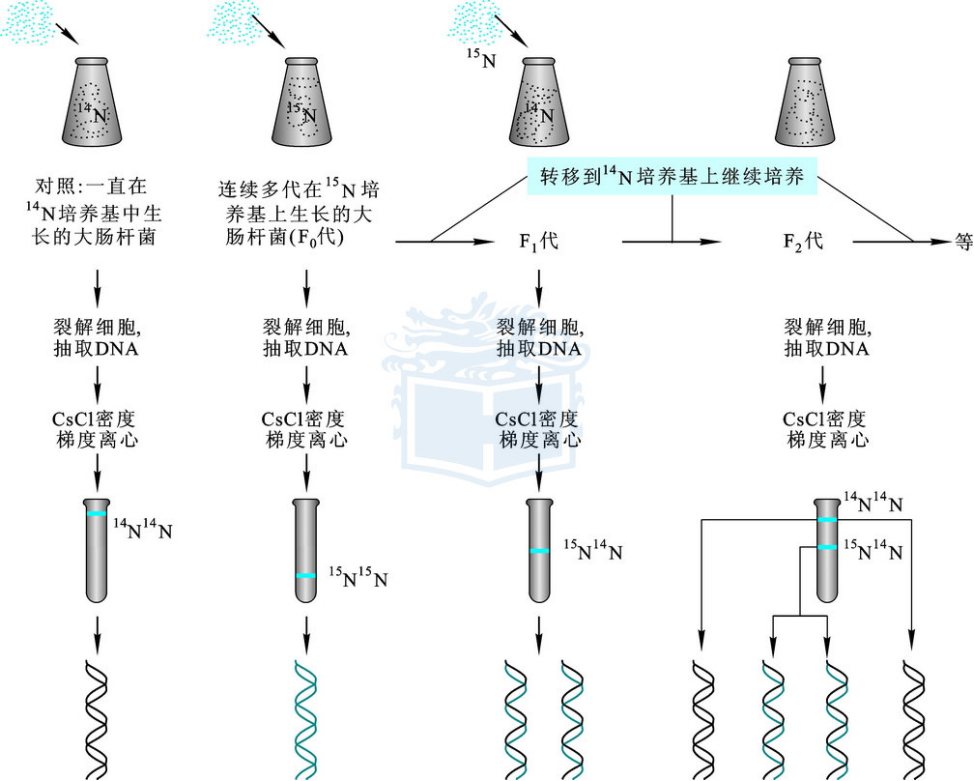
\includegraphics[width=\linewidth]{证明DNA半保留复制的实验.png}
	\caption{Meselson和Stahl的证明DNA半保留复制的实验流程}
	\label{fig:Meselson和Stahl的证明DNA半保留复制的实验流程}
\end{figure}

\begin{figure}[htbp]
	\centering
	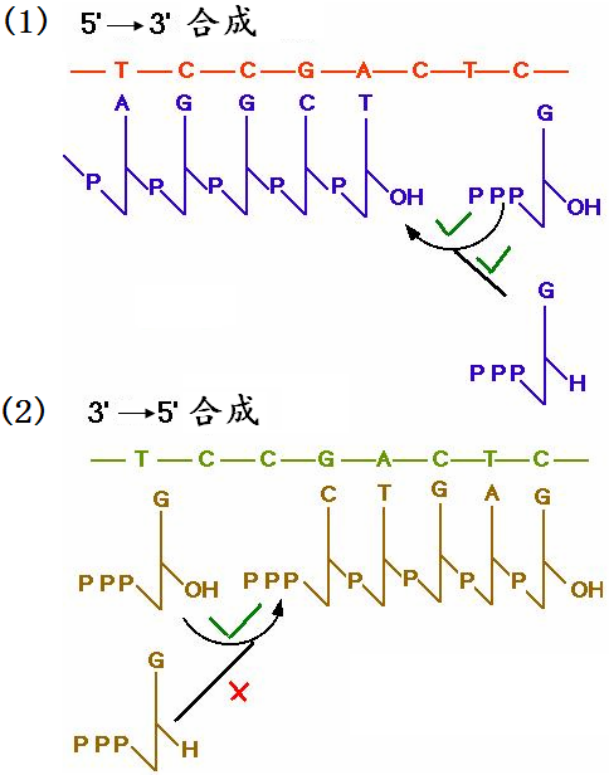
\includegraphics[width=0.4\linewidth]{证明DNA复制方向的实验.png}
	\caption{证明DNA复制方向的实验}
	\label{fig:证明DNA复制方向的实验}
\end{figure}

\subsubsection{不需要引物的生物}

DNA复制需要引物的生物学意义是,利于形成稳定的双螺旋结构,保证后续复制的忠实性。而这种在深海火山口附近细菌内的噬菌体,希望引入更多的突变,以求获得有利于生存的性状。

这种噬菌体编码的DNA聚合酶同时具有引发酶、DNA聚合酶、RNA聚合酶的特性。

\subsubsection{复制起始区和复制子}

复制起始区是作为DNA复制起点的一段碱基序列,具有如下特点:
\begin{description}
	\item[多个短的重复序列]
	\item[被复制起始区结合蛋白识别] 如DnaA(细菌)、Orc1-Orc6(真核)、Orc1/Cdc6(古菌)。
	\item[富含AT碱基对] AT碱基对之间只有2条氢键,比GC(3条)少,有利于解链。
\end{description}

细菌的DNA复制起始区只有一个,而真核生物和部分古菌有多个。

每个复制起始区构成一个复制子。DNA复制时,解链形成复制叉。(\autoref{fig:复制叉})

\begin{figure}[htbp]
	\centering
	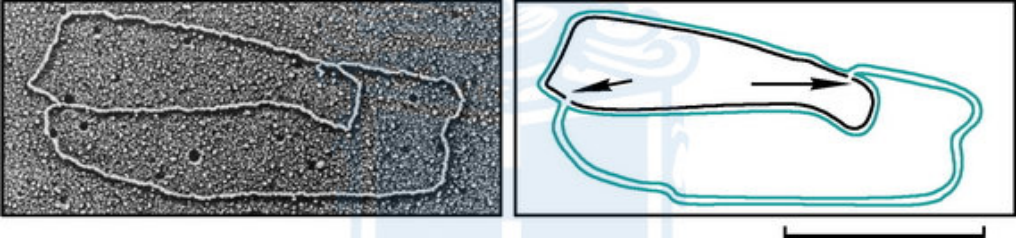
\includegraphics[width=0.7\linewidth]{复制叉.png}
	\caption{复制叉}
	\label{fig:复制叉}
\end{figure}

\subsection{参与DNA复制的主要酶和其他蛋白质}

DNA复制主要涉及DNA聚合酶、DNA解链酶、单链DNA结合蛋白、DNA引发酶、DNA拓扑异构酶、DNA连接酶、端粒酶等。

\subsubsection{DNA聚合酶}

DNA聚合酶,全名是依赖于DNA的DNA聚合酶(DNAP)。反应把dNTP转变成dNMP和PPi,相当于消耗了两个ATP。

DNA聚合酶的共性:

\begin{itemize}
	\item 不能催化DNA的从头合成,故DNA复制需要引物;
	\item 只能催化DNA从5$\prime$$\longrightarrow$3$\prime$合成;
	\item 类似于右手的构象:手指、手掌、拇指三个结构域;
	\item 都需要2个\ce{Mg^2+},一个随\ce{dNTP}进入活性中心、另一个本来就在那里。它们与活性中心的3个Asp残基结合。所有物种中,这3个Asp残基都是高度保守的;
\end{itemize}

	根据序列同源性,生物的DNAP可分为下面这些家族:(\autoref{tab:DNAP_family})
	\begin{table}[htbp]
		\centering
		\begin{tabularx}{\textwidth}{|c|l|X|}
			\hline
			\textbf{家族} & \multicolumn{1}{c|}{\textbf{存在生物}} & \multicolumn{1}{c|}{\textbf{代表DNA聚合酶}} \\ \hline
			A类 & 噬菌体、真核生物线粒体、细菌 & T7噬菌体、线粒体$\upgamma$、细菌I \\ \hline
			B类 & 细菌、古菌、真核生物 & 真核$\upalpha$、$\updelta$、$\upvarepsilon$、噬菌体T4和$\upPhi$29 \\ \hline
			C类 & 细菌 & 细菌III \\ \hline
			D类 & 古菌 &  \\ \hline
			X类 & 真核生物 & $\upbeta$、$\uplambda$、$\upmu$ \\ \hline
			Y类 & 真核生物、细菌 & 真核$\upeta$、$\upiota$、$\upkappa$、Rev1、细菌IV和V \\ \hline
			RT类 & 广泛存在 & 真核端粒酶、病毒逆转录酶 \\ \hline
		\end{tabularx}
		\caption{DNA聚合酶七大家族}
		\label{tab:DNAP_family}
	\end{table}

\subsubsection{DNA解链酶}

DNA解链酶就是催化DNA双螺旋解开的酶。任何一种DNA解链酶都可以序列无关地结合DNA,大多数解链酶优先结合DNA单链区域。

DNA解链酶具有下列酶活性:
\begin{description}
	\item[移位酶] 这使得DNA解链酶可以在DNA链这个轨道上移动(\ref{fig:Dnab});
	\item[ATP酶] 解链需要打破氢键、碱基堆积力,这需要ATP提供能量。
\end{description}

\begin{figure}
	\centering
	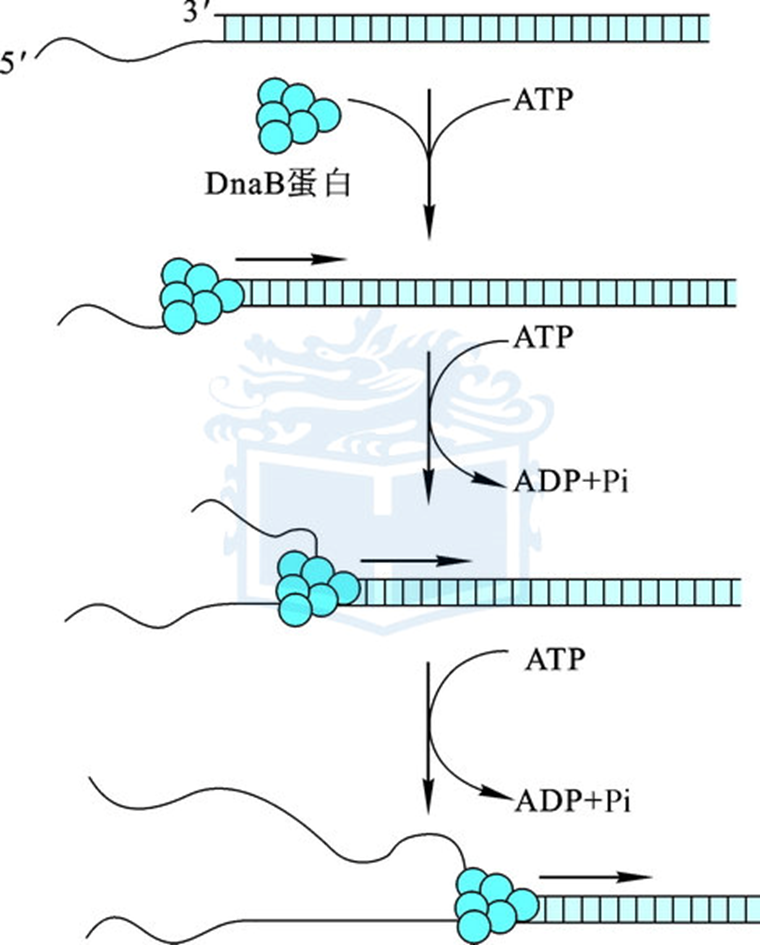
\includegraphics[width=0.5\linewidth]{Pics/DnaB}
	\caption{DnaB蛋白的移位酶活性}
	\label{fig:Dnab}
\end{figure}


在体外,我们使用热变性让DNA两条链分开,如在PCR中DNA的变性。

\subsubsection{单链结合蛋白(SSB)}

SSB专门与DNA单链区域结合,本身并没有酶活性。它具有以下功能:\begin{itemize}
	\item 维持DNA的单链状态,防止互补碱基重新配对;
	\item 防止DNA自发形成链内双螺旋,防止DNA聚合酶进行性因链内双螺旋受到影响;
	\item 包被单链DNA区段,防止核酸酶的水解;
	\item 刺激某些酶的活性。
\end{itemize}

SSB与DNA的结合还具有协同效应,就是说,当第一个SSB与DNA结合后,后面来的SSB就会更容易与DNA结合。

利用SSB与DNA单链的特异性结合,可以设计蛋白质纯化的方法。将目的蛋白和SSB融合表达,再将含融合蛋白的细胞裂解液通过与DNA交联的树脂,融合蛋白就被吸附在树脂上,后续进行洗脱即可。

\subsubsection{DNA拓扑异构酶}

如前述,DNA形成正超螺旋时,不利于解链,也就不利于复制;形成负超螺旋时,有利于解链和复制。所以,无论真核还是原核生物,在DNA尚未复制时,都是正超螺旋;DNA复制时,就变为负超螺旋。

DNA复制时,前面的DNA解链,后面的DNA就被挤成了正超螺旋(\autoref{fig:dna_positive_supercoiling})。这时就需要DNA拓扑异构酶出手了(\autoref{fig:DNA_topoisomerase})。

\begin{figure}[h]
	\centering
	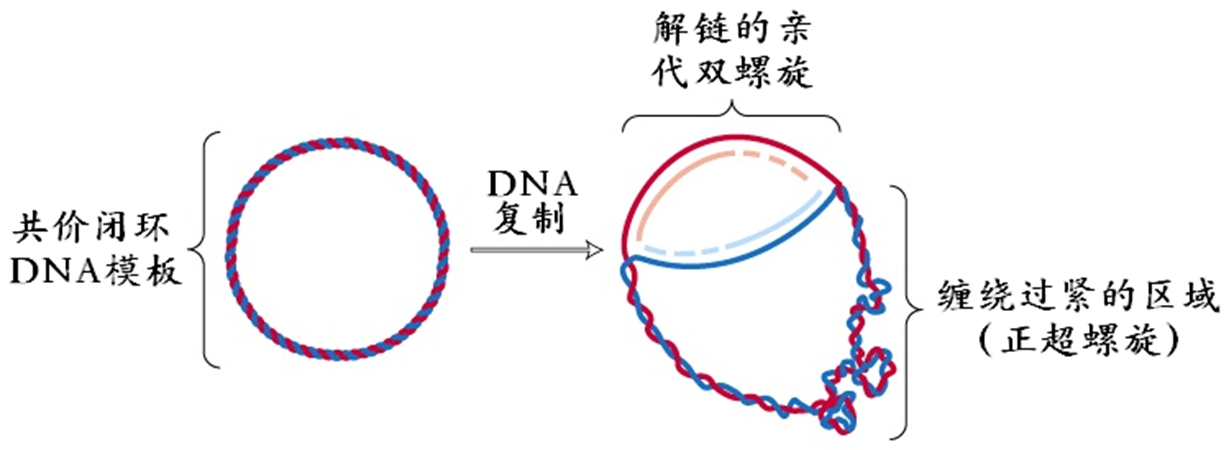
\includegraphics[width=0.7\linewidth]{Pics/DNA形成正超螺旋}
	\caption{DNA复制过程中形成的正超螺旋结构}
	\label{fig:dna_positive_supercoiling}
\end{figure}

\begin{figure}[h]
	\centering
	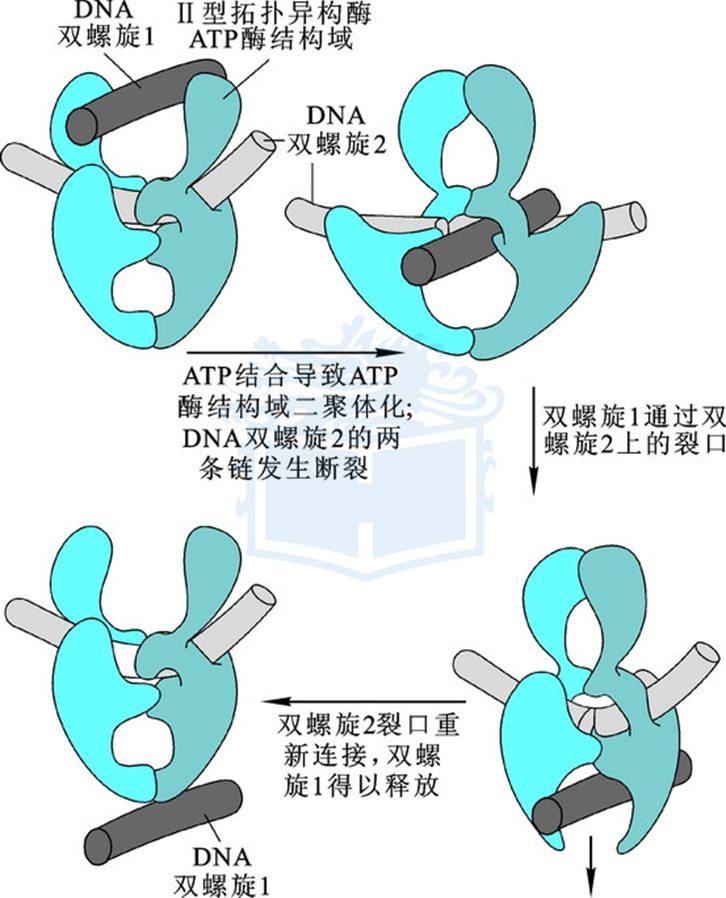
\includegraphics[width=0.7\linewidth]{Pics/DNA拓扑异构酶}
	\caption{II型DNA拓扑异构酶作用机制}
	\label{fig:DNA_topoisomerase}
\end{figure}

所有DNA拓扑异构酶的作用都是通过两次转酯反应完成的。酶的活性中心有一个Tyr残基,其羟基亲核进攻DNA主链上的3',5'-磷酸二酯键,使DNA发生断裂。断裂后,DNA拓扑学结构发生变化。做完这件事,拓扑异构酶就催化逆反应,把DNA重新接上。(\autoref{fig:DNA_topoisomerase_mechanism})

\begin{figure}[h]
	\centering
	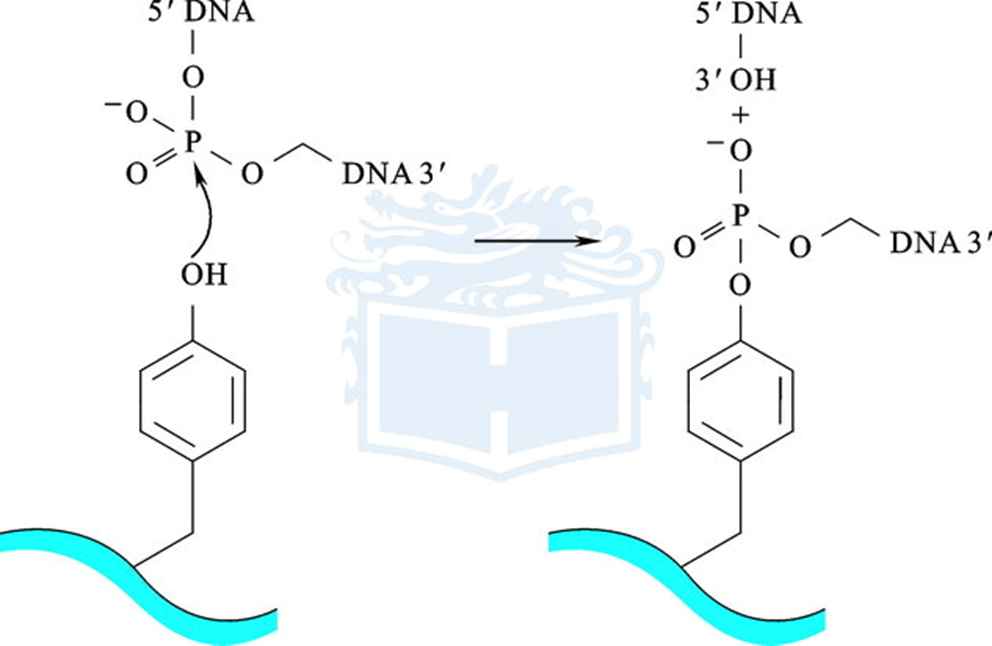
\includegraphics[width=0.7\linewidth]{Pics/DNA拓扑异构酶机理}
	\caption{DNA拓扑异构酶催化的转酯反应}
	\label{fig:DNA_topoisomerase_mechanism}
\end{figure}

DNA拓扑异构酶有不同类型,性质有所不同(\autoref{tab:dna_topoisomerase_subclass})。参与DNA复制的主要是II类。

细菌的旋转酶就属于II类DNA拓扑异构酶,A、B亚基各2个。环丙沙星抑制A亚基,抑制ATP酶活性;新生霉素作用于B亚基,增强旋转酶切断DNA酶的能力、抑制DNA链的重新连接。

喜树碱可以抑制真核生物的DNA拓扑异构酶,可以用于治疗癌症。

\begin{table}[htbp]
	\centering
	\begin{tabular}{|>{\centering\arraybackslash}m{7em}|>{\centering\arraybackslash}m{5em}|>{\centering\arraybackslash}m{5em}|>{\centering\arraybackslash}m{5em}|>{\centering\arraybackslash}m{5em}|}
		\hline
		分类 & \multicolumn{2}{c|}{I} & \multicolumn{2}{c|}{II} \\ \hline
		亚类 & IA & IB & IIA & IIB \\ \hline
		\ce{Mg^2+}的依赖性 & √ & × & √ & √ \\ \hline
		ATP的依赖性 & × & × & √ & √ \\ \hline
		切开DNA的几条链 & 1 & 1 & 2 & 2 \\ \hline
		切口与酶的连接方式 & 5'-磷酸酪氨酸酯键 & 3'-磷酸酪氨酸酯键 & 5'-磷酸酪氨酸酯键 & 5'-磷酸酪氨酸酯键 \\ \hline
		连环数的变化 & $\pm 1$ & 任何整数 & $\pm 2$ & $\pm 2$ \\ \hline
	\end{tabular}
	\caption{DNA拓扑异构酶的亚类和性质}
	\label{tab:dna_topoisomerase_subclass}
\end{table}

\subsubsection{DNA引发酶}

DNA引发酶是特殊的RNA聚合酶,负责RNA引物的合成。由于DNA复制具有半不连续性,所以DNA引发酶在前导链上只需要引发一次,在后随链上要引发多次。

大肠杆菌的引发酶为DnaG蛋白,真核细胞的引发酶在体内和DNA聚合酶$\upalpha$紧密结合在一起。真核细胞合成的引物短一些。

\subsubsection{切除引物的酶}

RNA引物在DNA复制完之后就要被切除。

细菌切除引物的酶是DNA聚合酶I或核糖核酸酶H(RNase H)。DNA聚合酶I利用自身5'外切酶活性切除引物;RNase H专门水解和DNA杂交(Hybrid)的RNA,其中就包含RNA引物。

真核生物没有兼职切引物的DNA聚合酶。RNase H1/FEN1这两个酶配合在一起负责切除RNA引物。FEN1称为翼式内切酶,有5'外切酶和内切酶活性。一般认为,RNase H1切除引物,但是最后剩一个没切掉,由FEN1切除。

\subsubsection{DNA连接酶}

DNA连接酶识别DNA分子内相邻的3'-羟基和5'-磷酸,并催化形成3',5'-磷酸二酯键。有时甚至催化的是DNA分子两条链上的碱基相连。

DNA连接酶在DNA复制中,担当连接冈崎片段的任务。在DNA修复和重组中,则负责闭合DNA链上的切口。

DNA连接酶催化反应时消耗的能量来源于\ce{NAD+}或ATP。绝大多数细菌属于前者,少数细菌、所有真核生物、古菌、病毒属于后者。从\ce{NAD+}的结构就可以看出,它“相当于”一个ADP。

\subsubsection{端粒酶}

DNA每次复制,后随链上最后一个冈崎片段切除掉RNA引物后,就没有了下一次DNA复制起始,导致切掉的那一段空着了,反复下去就导致端粒\footnote{人的端粒重复序列是TTAGGG。}缩短。为了补上这一段缺失,需要端粒酶(\autoref{fig:telomere})。

\begin{figure}[h]
	\centering
	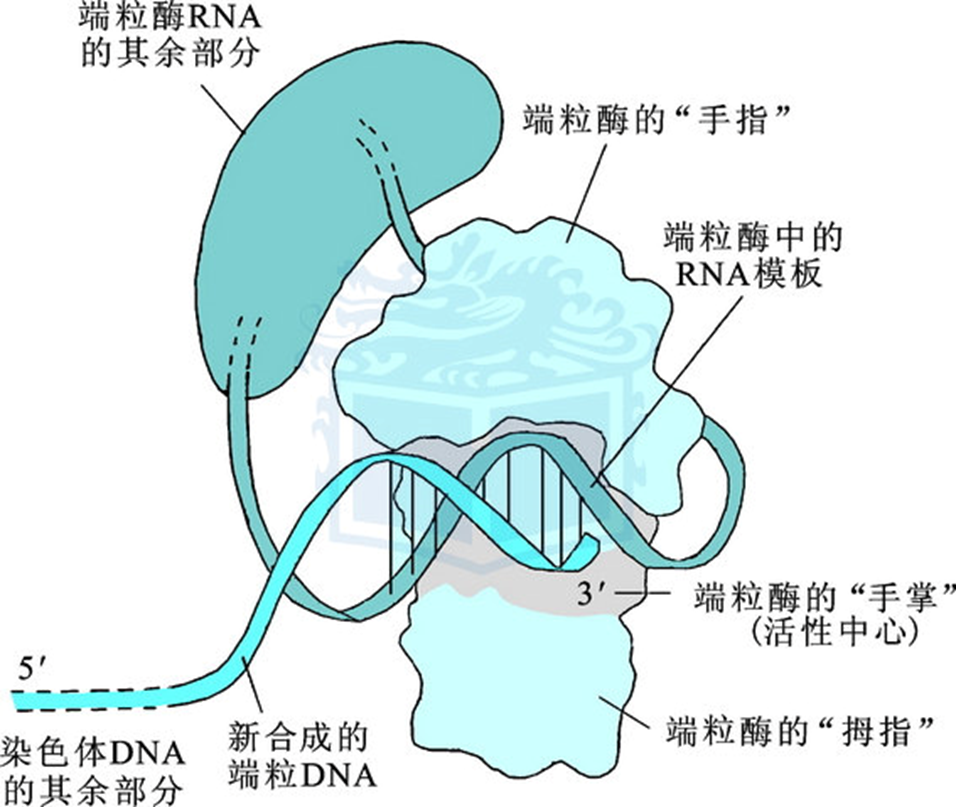
\includegraphics[width=0.5\linewidth]{Pics/端粒酶}
	\caption{端粒酶的结构}
	\label{fig:telomere}
\end{figure}


端粒酶是逆转录酶,含有蛋白质和RNA,RNA是逆转录的模板。

端粒酶作用机制见。需要注意的是,端粒酶并非直接延长变短的端粒,而是先延长模板链(老链),再由DNA聚合酶把变短的端粒补上。(\autoref{fig:telomere_mechanism})

\begin{figure}[h]
	\centering
	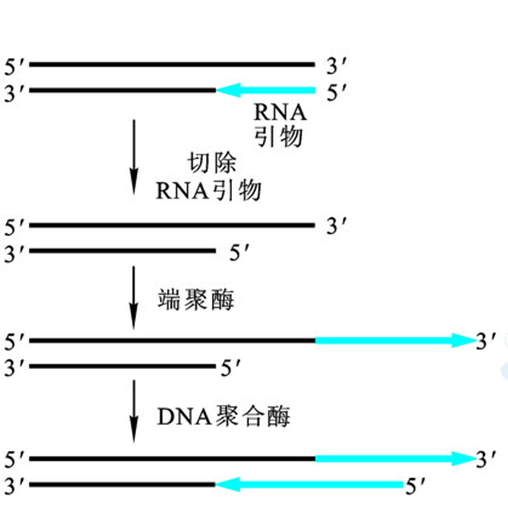
\includegraphics[width=0.4\linewidth]{Pics/端粒酶1}
	\caption{端粒酶的作用机制}
	\label{fig:telomere_mechanism}
\end{figure}

多细胞生物体内大多数体细胞都没有端粒酶活性,这是为了限制分裂次数,防止DNA突变的积累。体内,只有胚胎细胞、生殖细胞、癌细胞才有端粒酶活性。

对于单细胞真核生物,其体内端粒酶活性一直很高。这很显然,要不然它们早就灭绝了。

细菌、线粒体、叶绿体等具有环形DNA的生物(或结构),不需要端粒酶。

\subsection{DNA复制的详细机制}

DNA复制是以复制子为单位进行的。任何一个复制子都含有一个复制起始区,有的还含有终止区。

细菌、噬菌体、质粒、线粒体的基因组都只有一个复制子,真核细胞内每个染色体上的DNA都有多个复制子。

任何DNA复制过程,都可以人为分为起始、延伸和终止三个阶段。

\subsubsection{以大肠杆菌为代表的$\uptheta$复制}
\paragraph{DNA复制的起始}
这一阶段起始于对\textit{OriC}的识别,结束于引发体的形成。

\begin{longtable}[c]{|l|l|}
	\hline
	\multicolumn{1}{|c|}{蛋白质名称} & \multicolumn{1}{c|}{功能} \\ \hline
	\endfirsthead
	%
	\multicolumn{2}{l}{\textbf{续表}} \\
	\hline
	\multicolumn{1}{|c|}{蛋白质名称} & \multicolumn{1}{c|}{功能} \\ \hline
	\endhead
	%
	DNA旋转酶 & II型拓扑异构酶,负责清除复制叉前进中的拓扑学障碍 \\ \hline
	SSB & 单链结合蛋白 \\ \hline
	DnaA蛋白 & 复制起始因子,识别复制起始区\textit{OriC} \\ \hline
	DnaB蛋白 & DNA解链酶 \\ \hline
	DnaC蛋白 & 招募DnaB蛋白到复制叉 \\ \hline
	DnaG蛋白 & DNA引发酶,引物合成 \\ \hline
	DnaT蛋白 & 辅助DnaC蛋白的作用 \\ \hline
	HU蛋白 & 类似于真核细胞的组蛋白,结合DNA并使DNA弯曲 \\ \hline
	PriA蛋白 & 引发体的装配 \\ \hline
	PriB蛋白 & 引发体的装配 \\ \hline
	PriC蛋白 & 引发体的装配 \\ \hline
	DNA聚合酶III & DNA链的延伸 \\ \hline
	DNA聚合酶I & 切除引物,填补空隙 \\ \hline
	DNA连接酶 & 缝合相邻的冈崎片段 \\ \hline
	DNA拓扑异构酶IV & 分离子代DNA \\ \hline
	Tus & 复制终止
	 \\ \hline
	\caption{参与大肠杆菌DNA复制的主要蛋白质}
	\label{tab:ecoli_DNA_duplicatipn}
\end{longtable}





\section{DNA的损伤、修复和突变}

DNA是唯一一种在发生损伤后可以在体内被完全修复的分子,但也并不是所有情况都可以修复。流程是这样的:DNA发生损伤$\longrightarrow$尝试修复$\longrightarrow$修复不了就等于发生了突变,修复得了就一切正常。

细胞之所以这么重视DNA,是因为DNA只有有限的拷贝数,对于单倍体生物更是少得可怜。此外,DNA具有互补的双螺旋结构,使修复变得容易。
\subsection{DNA的损伤}

DNA损伤分为碱基损伤和DNA链损伤。

碱基损伤可如下分类:\begin{description}
	\item[碱基脱落] 原因是,化学上来说,$\upbeta$-N-糖苷键可以自发水解,碱基就掉下来了。脱嘌呤最普遍。
	\item[碱基转换] 一种碱基变为另一种碱基。成因可以是碱基自发地脱氨基,如C$\longrightarrow$U,A$\longrightarrow$I;可以是化学诱变剂或碱基类似物。
	\item[碱基修饰] 由某些化学试剂或活性氧造成的。如:鸟嘌呤$\xrightarrow{\text{硫酸二甲酯}}$\ce{O^6}-甲基鸟嘌呤、鸟嘌呤$\xrightarrow{\text{活性氧}}$8-氧鸟嘌呤。
	\item[碱基交联] 紫外线导致DNA上相邻的嘧啶碱基形成嘧啶二聚体,尤其是TT碱基。嘧啶二聚体包括环丁烷二聚体、4-6光产物两种类型(\autoref{fig:uv_damage})。
	\begin{figure}[h!]
		\centering
		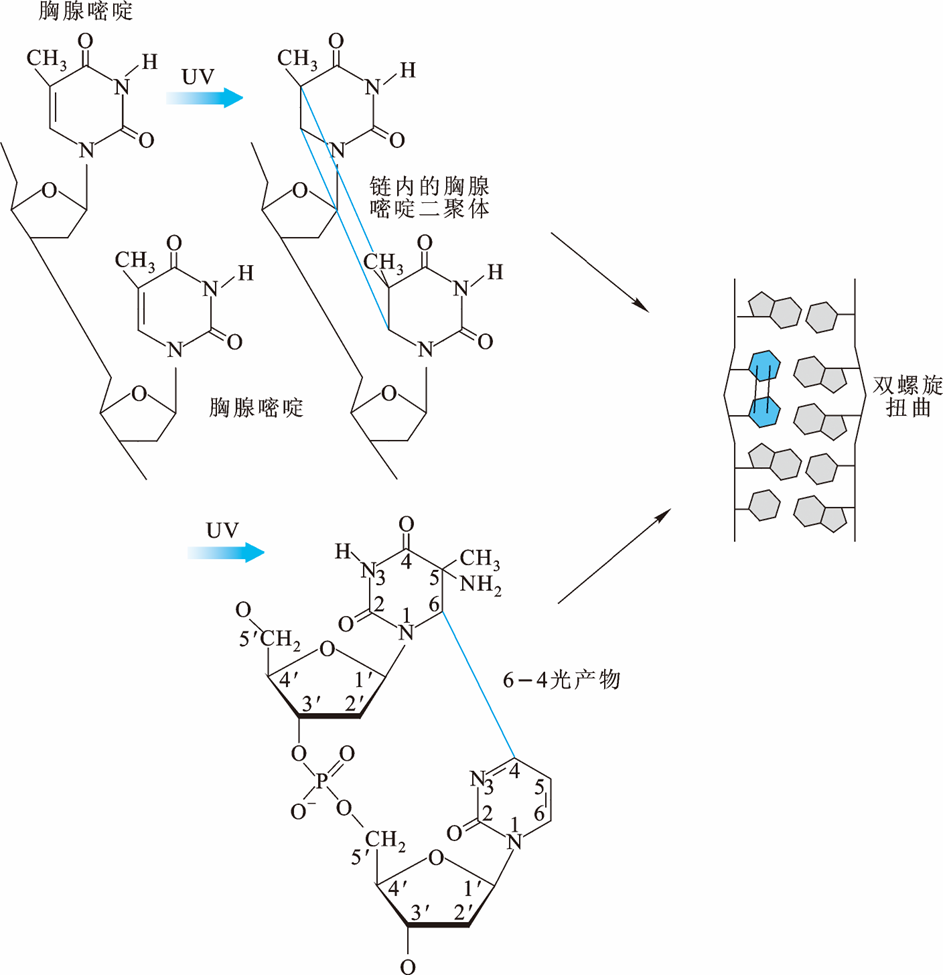
\includegraphics[width=0.7\linewidth]{4-6光产物和嘧啶二聚体}
		\caption{紫外线引发的碱基损伤}
		\label{fig:uv_damage}
	\end{figure}
	\item[碱基错配] DNA复制过程中,四种dNTP的浓度不平衡、碱基互变异构等等都有可能导致碱基错配。尽管大多数错配都会被DNA聚合酶修复,但仍然会有“漏网之鱼”。
\end{description}

DNA链损伤分为以下四类:\begin{description}
	\item[核糖核苷酸的掺入] 细胞中的NTP误入DNAP的活性中心导致的。
	\item[DNA链的有断裂] 有单链断裂和双链断裂两种类型。原因有离子辐射和某些化学试剂的作用,如博来霉素。这种损伤是最严重的,当DNA链出现太多裂口,尤其是双链断裂,难以修复,就会导致细胞凋亡。
	\item[DNA链间交联] 这是由于某些双功能试剂的使用,如丝裂霉素C和顺铂。
	\item[DNA与蛋白质交联] 甲醛或较强的紫外线可诱导DNA结合蛋白与DNA之间形成共价键。
\end{description}

\subsection{DNA的修复}

DNA修复可分为直接修复、切除修复、双链断裂修复和损伤跨越。

\subsubsection{直接修复}

直接修复是将损伤的碱基或者核苷酸直接逆转,而不是切除。能够这样被修复的有嘧啶二聚体和\ce{O^6}-烷基鸟嘌呤,此外,若DNA链在磷酸二酯键上断裂,且裂口是5'-磷酸和3'-羟基,那么DNA连接酶也会直接修复。

\paragraph{嘧啶二聚体的直接修复}

催化反应的酶是光裂合酶(光复活酶),分为两种:\begin{description}
	\item[第一类] 有两个辅基:\begin{enumerate}
		\item 以半醌形式存在的\ce{FAD-};
		\item 5,10-甲炔基-四氢叶酸(MTHF)或8-羟基-5-去氮黄素(8-HDF)。
	\end{enumerate}
	\item[第二类] 只有一个\ce{FAD-}辅基。
\end{description}
辅基的功能与光系统中的捕光色素类似,捕捉蓝光和近紫外光(\qtyrange{350}{450}{\nano\meter})。对于催化修复反应来说,只有\ce{FAD-}是必须的,另外的MTHF或8-HDF能在低光条件下提高反应速率。

大肠杆菌的光裂合酶可以结合单链或双链DNA,酶分子表面在结合DNA的地方有带正电的小孔,正好容纳嘧啶二聚体。嘧啶二聚体的出现使DNA链发生扭转、链间碱基的作用力减弱,也就使翻转过程变得容易。

\begin{wrapfigure}{r}{0.4\textwidth}
	\centering
	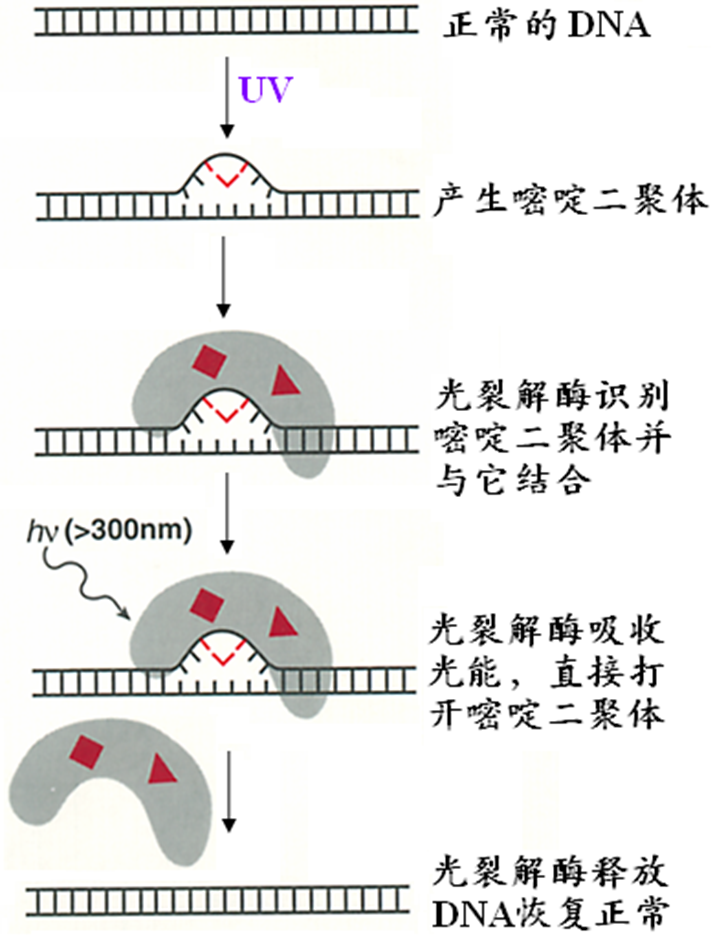
\includegraphics[width=\linewidth]{光裂合酶}
	\caption{光裂合酶的工作过程}
	\label{fig:photolyase}
\end{wrapfigure}

光裂合酶的作用过程分两步(\autoref{fig:photolyase}):\begin{enumerate}
	\item 酶直接识别、结合嘧啶二聚体,使其发生翻转落入活性中心,不需要光;
	\item 第一类光裂合酶的MTHF或8-HDF辅基吸光,把光能传给\ce{FAD-},第二类则是\ce{FAD-}直接捕获光能。\ce{FAD-}接收光能后失去一个电子,传给嘧啶二聚体,使它变得不稳定,最后二聚体之间的共价键被打破,电子又回来。\ce{FAD-}再生。
\end{enumerate}

光裂合酶广泛存在于细菌、古菌、真核生物中,甚至一些真核生物的线粒体、叶绿体,遗憾的是胎盘类哺乳动物没有。但是在人和其他哺乳动物体内发现了光复活酶的同源蛋白——隐蔽色素(CRY)。它们具有\ce{FAD-}和捕光色素,但没有光裂合酶的活性,可能是光信号的受体,参与生物钟的调节。

\paragraph{烷基化碱基的直接修复}

酶是烷基转移酶,以\ce{O^6}-甲基鸟嘌呤甲基转移酶(MGMT)最常见。它是“自杀式催化” 的(\autoref{fig:alkyltranseferase})。

\begin{wrapfigure}{r}{0.3\textwidth}
	\centering
	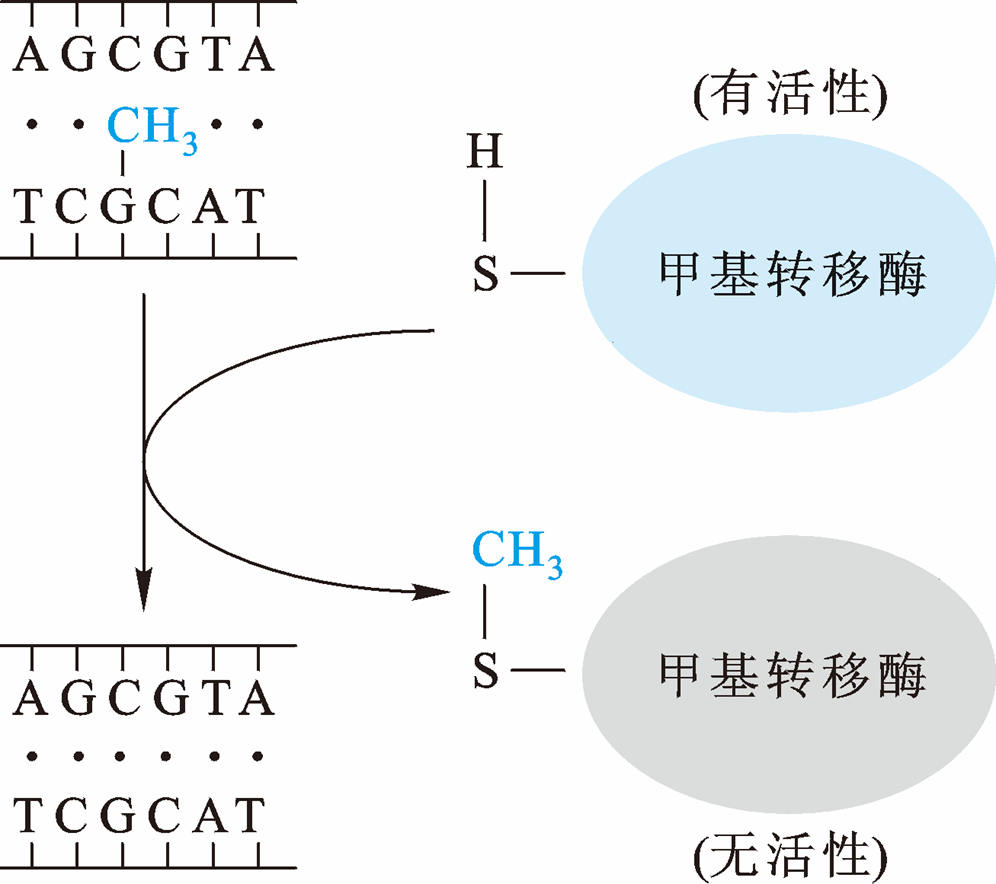
\includegraphics[width=\linewidth]{烷基转移酶}
	\caption{烷基化碱基的直接修复}
	\label{fig:alkyltranseferase}
\end{wrapfigure}

甲基转移酶的Cys残基得到甲基后就失活了,随后被泛素化降解。该酶是一种诱导酶。

\subsubsection{切除修复}

切除修复就是切除受损的碱基或核苷酸,然后重新合成正常的碱基或核苷酸,再经连接酶把接口缝合。整个修复过程包括识别、切除、重新合成、重新连接四步(4R)。

切除修复分为:\begin{description}
	\item[碱基切除修复(BER)] 直接识别受损伤的碱基;
	\item[核苷酸切除修复(NER)] 识别损伤对DNA双螺旋结构的扭曲,这意味着损伤更严重。
\end{description}
BER和NER的选择,就在于损伤的性质。

\paragraph{碱基切除修复(BER)}

\begin{figure}[h!]
	\centering
	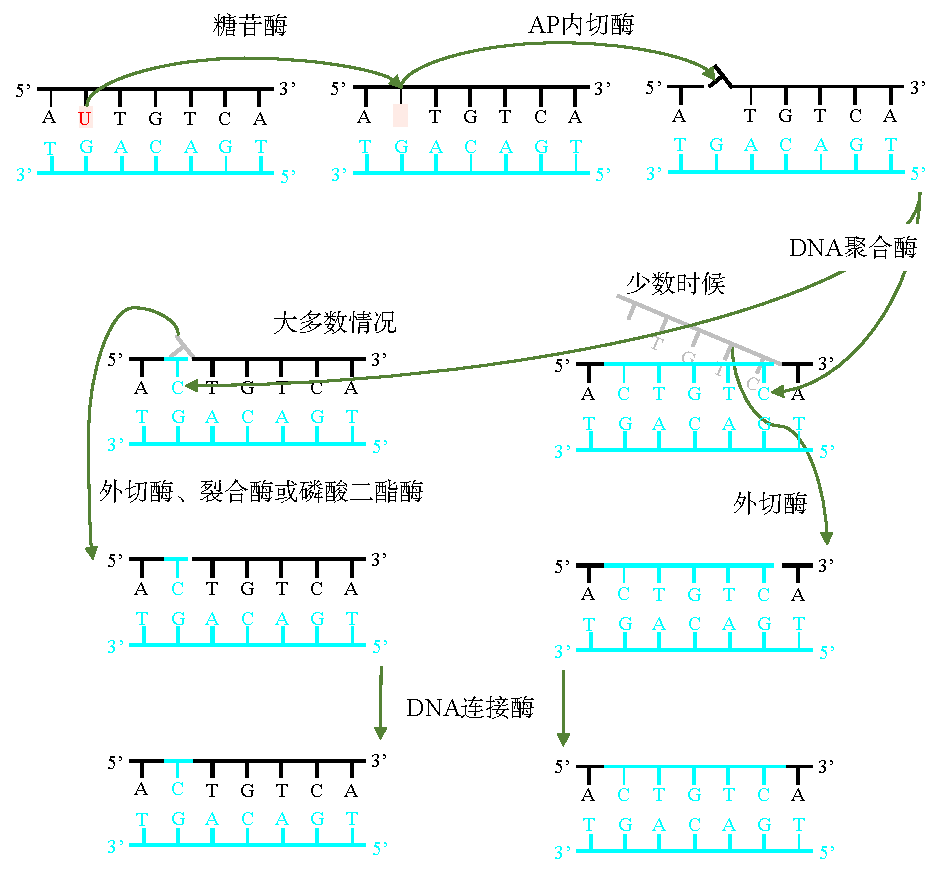
\includegraphics{尿嘧啶BER.pdf}
	\caption{尿嘧啶的切除修复}
	\label{fig:ber}
\end{figure}


\paragraph{核苷酸切除修复(NER)}

NER用于修复
NER分为全局NER(GGR)和转录偶联性NER(TCR)。

\paragraph{错配修复(MMR)}


\section{DNA重组}

\section{DNA转录}

细胞内主要含有的RNA有三种:mRNA、tRNA、rRNA,此外还有一些小RNA,如真核细胞内的miRNA、snRNA、7SL RNA。这些RNA都能与DNA杂交,表明它们都是转录出来的。

\subsection{DNA转录的一般特征}

DNA转录可以发生在细胞内,包括细胞质基质(原核生物、古菌)、细胞核(真核生物)、线粒体基质、叶绿体基质,也可以发生在体外。

DNA转录有以下共同特征:

\begin{enumerate}
	\item 转录有选择性和不对称性。不同于DNA复制,对于一个基因而言,只有一条DNA链作为转录模板,称模板链,而且一个基因的转录并非时刻都在进行、不同基因未必都以同一条链作模板链。

	模板链和非模板链相对,它们有一些别名:(\autoref{tab:template_strand})

	\begin{table}[h!]
		\centering
		\begin{tabular}{|c|l|c|}
			\cline{1-1} \cline{3-3}
			\textbf{模板链} & ~ & \textbf{非模板链} \\ \cline{1-1} \cline{3-3}
			非编码链 &  & 编码链 \\ \cline{1-1} \cline{3-3}
			无义链 &  & 有义链 \\ \cline{1-1} \cline{3-3}
			Waston链 &  & Crick链 \\ \cline{1-1} \cline{3-3}
		\end{tabular}
		\caption{模板链和非模板链的别名}
		\label{tab:template_strand}
	\end{table}

	\item 以四种NTPs为原料,需要2个\ce{Mg^2+}。
	\item 转录需要模板、解链,但不需要引物。
	\item 最先转录出来的通常是嘌呤碱基。
	\item 转录也有高度忠实性,但比DNA复制低。
	\item 方向和DNA复制一样,从5'$\rightleftharpoons$3'。
	\item 高度的进行性。意思是说,RNA聚合酶一旦结合,在转录终止前就不再脱落,万一酶从模板上解离,就再也不会重新结合。
	\item 转录受到严格调控。
\end{enumerate}

\subsection{RNA聚合酶}

转录起主导作用的是RNA聚合酶,全名叫依赖于DNA的RNA聚合酶。催化的反应通式为:
\[
n\text{NTPs}\xrightarrow[\text{RNA聚合酶}]{\text{DNA模板},\ce{Mg^2+}}(\text{NMP})_{n}+\text{PPi}
\]

反应机制与DNA聚合酶极为相似,再次提醒,这里生成PPi,相当于是两个ATP的能量。

这两类聚合酶仍有一些差别,下面详述:
\begin{enumerate}
	\item RNA聚合酶只有5'$\longrightarrow$3'聚合酶活性,无3'外切酶活性,这使得转录的忠实性不如DNA复制。但是RNA聚合酶具有“潜在的”内切酶活性,下面分开来讲:
	\begin{itemize}
		\item 活性中心本来就具有内切酶活性,如真核细胞的RNA聚合酶I;
		\item 与特定的转录因子结合,组装成完整的内切酶活性中心,如细菌的RNA聚合酶、真核细胞的RNA聚合酶II。
	\end{itemize}
	\item RNA聚合酶自带解链酶活性。
	\item RNA聚合酶不需要引物。
	\item 转录起始阶段,RNA聚合酶会催化几次无效转录,即RNA聚合酶在离开启动子进入转录延伸阶段之前,会反复启动转录,并释放出很短的无用转录物。
	\item 在转录起始阶段,DNA会在RNA聚合酶的活性中心形成褶皱,保证RNA聚合酶在进行无效转录时,仍能与启动子结合。
	\item 转录过程中,RNA产物不断与模板解离。
	\item RNA聚合酶在转录起始阶段受到多种调节蛋白的调控。
	\item 底物是NTP而不是dNTP。有U,无T。RNA聚合酶可以识别核糖环上的2'-OH,以此区分NTP和dNTP。
	\item 启动转录需要识别启动子。
	\item 反应速率低。
\end{enumerate}

\subsubsection{细菌的RNA聚合酶——以大肠杆菌为例}

大肠杆菌的RNA聚合酶有核心酶和全酶两种形式,核心酶的组成为$\upalpha_2\upbeta\upbeta'\upomega$,其中$\upbeta'$亚基结合有2个\ce{Mg^2+}。$\text{全酶}=\text{核心酶} + \upsigma\text{因子}$各亚基功能见\autoref{tab:ecoli_RNAP}。

\begin{table}[h]
	\centering
	\begin{tabular}{|c|c|c|c|m{15em}|}
		\hline
		\textbf{亚基} & \textbf{基因} & \textbf{分子量($\displaystyle\times 10^{3}$)} & 数目/酶 & \multicolumn{1}{c|}{\textbf{功能}} \\ \hline
		$\upalpha$ & \textit{RopA} & 36 & 2 & 核心酶的组装,转录起始,与调节蛋白的作用 \\ \hline
		$\upbeta$ & \textit{RopB} & 151 & 1 & 转录的起始和延伸 \\ \hline
		$\upbeta'$ & \textit{RopC} & 155 & 1 & 与DNA非特异性结合 \\ \hline
		$\upomega$ & \textit{RopZ} & 11 & 1 & 促进核心酶的组装,为β′亚基的分子伴侣,在体外为变性的RNA聚合酶成功复性所必需 \\ \hline
		$\upsigma_{70}$ & \textit{RopD} & 70 & 1 & 启动子的识别 \\ \hline
	\end{tabular}
	\caption{大肠杆菌RNA聚合酶的组成}
	\label{tab:ecoli_RNAP}
\end{table}

